\documentclass[11pt,unknownkeysallowed,usenames,dvipsnames]{beamer}
\usepackage[utf8]{inputenc}
\usetheme{metropolis}

% A font that I found more "classy" than the default one ...
% -- just comment the three next lines if you hate it ;)
\usepackage{libertine}
\renewcommand*\familydefault{\sfdefault}
\usepackage[T1]{fontenc}

% Packages
\usepackage{amsmath}
\usepackage{hyperref}
\hypersetup{colorlinks,breaklinks,
    urlcolor=teal,linkcolor=teal,citecolor=teal}
\graphicspath{{img/}}

% Beamer settings
\setbeamercolor{block title}{bg=gray!30}
\setbeamercolor{block body}{bg=gray!10}
\setbeamersize{text margin left=16pt,text margin right=16pt}

% Set minted options
\usepackage{minted}
\usepackage{anyfontsize}
\usepackage{t1enc}
\newminted{python}{fontsize=\fontsize{7}{8}\selectfont, 
    linenos=false,
    numbersep=8pt,
    gobble=0,
    bgcolor=gray!10,
    fontfamily=courier}

% Title and ...
\title{An (other one) introduction to Python}
\author{Thibaut Lunet}

\date{April 1, 2019}

\begin{document}
	\maketitle
    
	\begin{frame}{What are we talking about}
        \begin{block}{A little bit of history}
            \begin{itemize}
            \item Programming language conceived by a Monty Python fan in the 80's
            \item First released in 1991, then
            \begin{itemize}
                \item Python 2 in 2000 (community backed development, support $\rightarrow$ 2020)
                \item Python 3 in 2008 (major revision)
            \end{itemize}
            \end{itemize}
            Current versions (2.7, 3.6) are not entirely compatible, 
            but very close
        \end{block}
        
        \begin{block}{Main motivations}
            Developers wanted to create a language that would be
            
            \vspace{-10pt}
            \begin{itemize}
                \item general purpose (they really got that !)
                \item highly extensible and modular (dynamic language)
                \item beautiful, simple, easily readable
               \end{itemize} 
        \end{block}
        
        \vspace*{-20pt}
	\end{frame}
    
	\begin{frame}{Functioning principles}
        \begin{block}{Pre-compilation of code files}
            \centering
            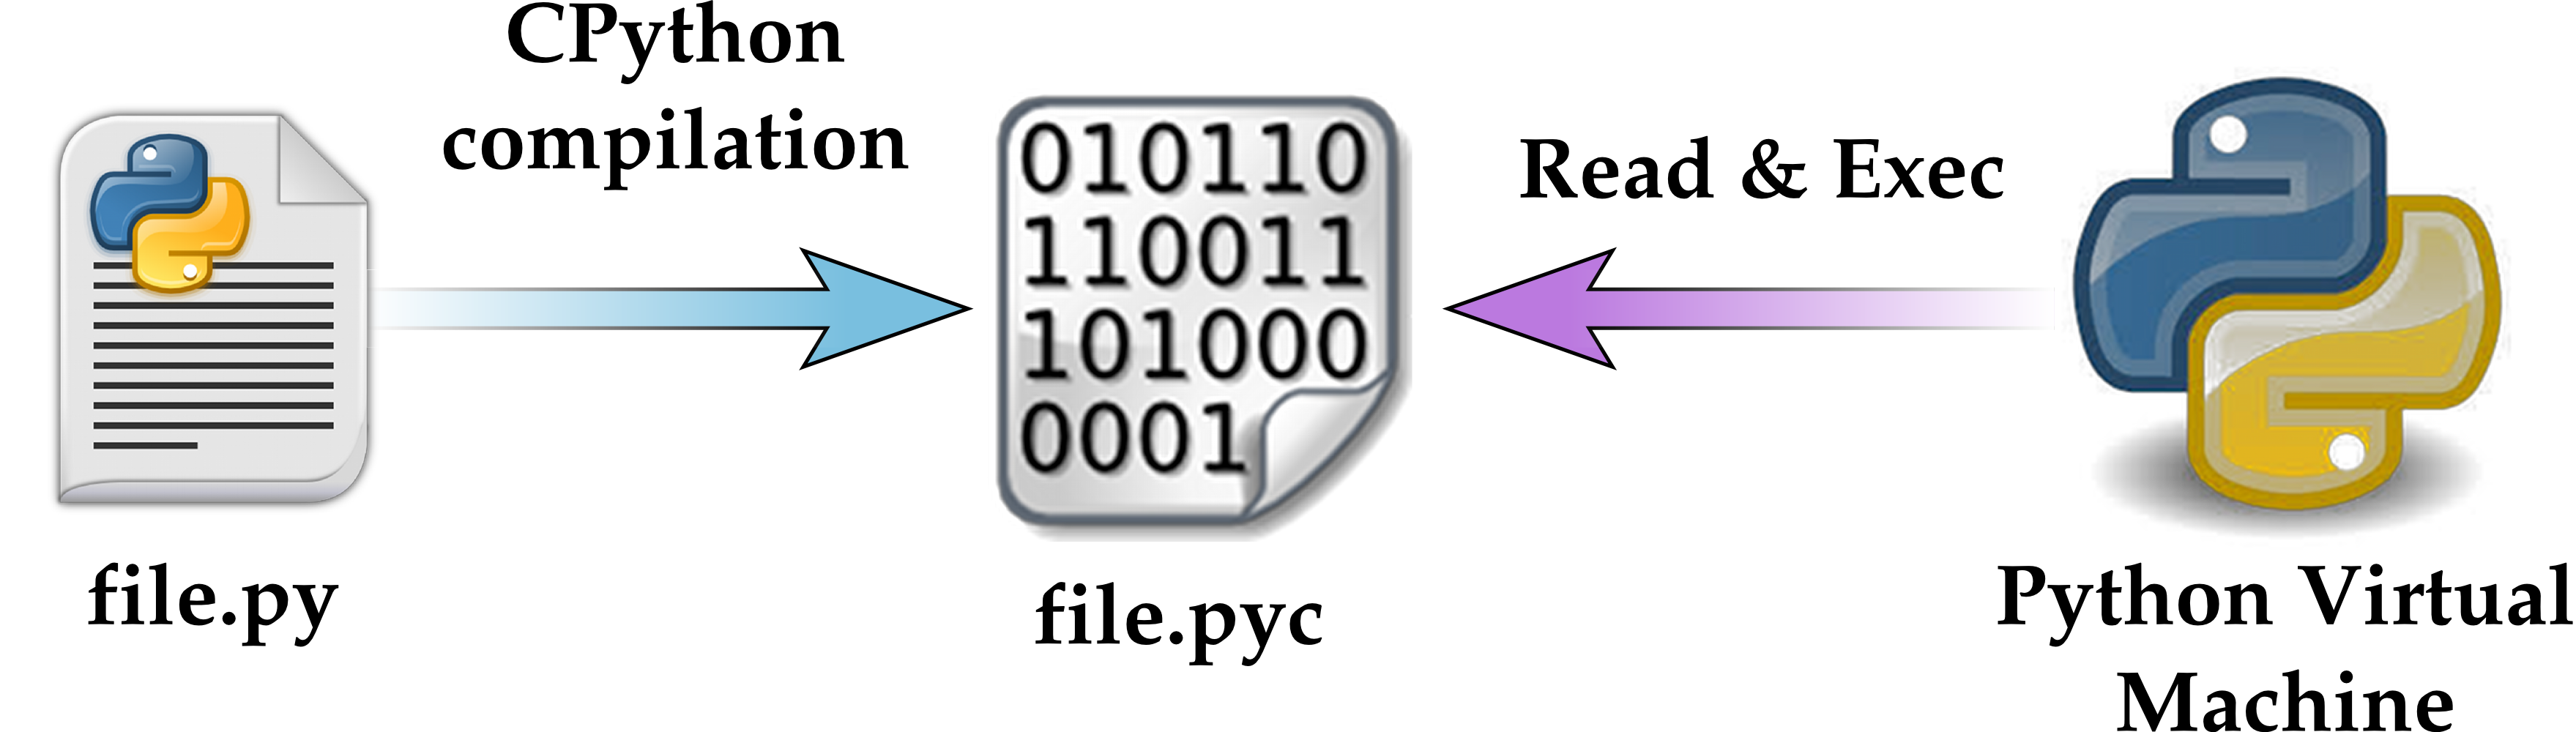
\includegraphics[width=0.8\linewidth]{cpython}
            
            \vspace*{-20pt}   
            \begin{itemize}
                \item Allows partial code optimization
                \item Totally transparent to user
                \item Portability on every architecture
            \end{itemize}
        \end{block}
        Python core (Virtual Machine) is written in C:
        
        \vspace*{-5pt}
        \begin{itemize}
            \item Easy interface with other compiled languages (C/C++, Fortran)
            \item Same speed as C when reading/writing files
        \end{itemize}
        
        \vspace*{-20pt}
    \end{frame}

	\begin{frame}{Python vs. Others (Matlab, Fortran, C/C++, ...)}
        \begin{itemize}
            \item License-free and open-source ($\neq$ Matlab)
            \item Huge users community, many (free) packages for many applications
            \item Extremely easy of use for non-I-love-programming people \\ (no compilation, no variable declaration, ... $\neq$ Fortran, C/C++)
            \item Computation can be accelerated using Fortran or C/C++
            library ... 
            \item Can scale to very large problems (parallel computing, ...)
            \item Structured and friendly ways for developing library ($\neq$ Matlab)
        \end{itemize}
		\begin{tabular}{rl}
			Python&$=$ excellent solution for algorithm development and prototyping\\
			&$\neq$ solution for fast and memory-optimized production codes
		\end{tabular}
	\end{frame}

\begin{frame}{Two particular aspects}
\vspace*{5pt}
\begin{block}{Implementation is based on indentation}
	Each code block (condition, loop, function definition, ...) 
	are delimited by indentation, not by brackets or "end ..." commands
	\begin{itemize}
		\item Strange, but also ease implementation
		\item Forces to write well presented codes
	\end{itemize}
\end{block}
\vspace*{5pt}
\begin{block}{Everything is object}
	Every programming elements (type, lists, function, ...) are objects, 
	i.e they have their own attributes and methods
	\begin{itemize}
		\item Induces a particular call of functions ("result = object.function(...)")
		\item Object Oriented programming is natural
		\item Classical way of calling function ("res = function(...)") still available
	\end{itemize}
\end{block}
\end{frame}

\begin{frame}{How to use Python}
    \vspace{5pt}
    \begin{block}{Basic use : script and terminal}
    Code is written in text files, and run using the "python" terminal command
    \begin{center}
    	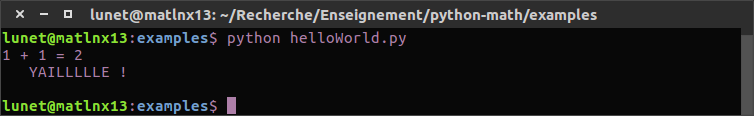
\includegraphics[width=0.95\linewidth]{python-script}
    \end{center}
	\begin{itemize}
		\item Need to know how to open a terminal 
		(in Ubuntu, Windows, Mac, ...)
		\item Line by line command can be executed through the "python" or "ipython" commands
	\end{itemize} 
    \end{block}
\end{frame}

\begin{frame}{How to use Python}
	\vspace*{5pt}
    \begin{block}{Advanced use : the Spyder Developing Environment}
	Graphical interface program ($\sim$ Matlab, Mathematica, ...)
	\vspace*{-10pt}
	\begin{center}
		
\includegraphics[width=0.24\linewidth]{spyder-logo}%
	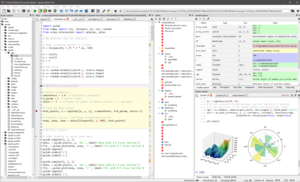
\includegraphics[width=0.4\linewidth]{spyder-screensho}
	\end{center}
	\vspace*{-10pt}
	\begin{itemize}
		\item Writing and running scripts interactively
		\item Dynamical access to variable
		\item Easy-access documentaion
		\item Automatic completion
		\item ...
	\end{itemize}
\end{block}
\end{frame}

\defverbatim[colored]\pythonCode{
\begin{pythoncode}     
# Lines starting with # are comments
print('I can do it !')

# Some first examples to run yourself
a = 1.2345
b = 2
print('a+b=', a+b)
\end{pythoncode}
} 
\begin{frame}{Spyder demonstration, and hands-on examples}
\begin{itemize}
	\item Installation of Python and Spyder using Anaconda distribution\\
	\href{https://www.anaconda.com/distribution}{https://www.anaconda.com/distribution} $\Rightarrow$ install Python 3.7
	\item Launch Spyder, and open a script file in the editor
	\item Test with the following examples, by running the script or typing those commands in the ipython terminal
\end{itemize}
\pythonCode
$\rightarrow$ try to find a and b variables in the variable editor
\end{frame}

\defverbatim[colored]\pythonCode{
\begin{pythoncode}     
# Integer
n = 1
m = 7 % 3  # modulo operator, m = 1
k = 7 // 2  # integer division, k = 3
i = int(1.7)  # integer conversion with built-in function, i = 1

# Float: by default, double precision
x = 0.5
y = x/7  # y = 0.07142857142857142
t = float('4.35')  # float conversion, t = 4.35 

# Complex
z = 1+1j
w = z + x + n  # Automatic conversion, w = 2.5 + 1j
c = complex(1, 5)  # Other definition, c = 1+5j

# Boolean
p = True
q = (n != 1)*p + (n == 1)*(x < 10)*(y >= 0)  # q = True = 1
r = bool(5)  # Alternative definition, False only for 0 or None
\end{pythoncode}
} 
\begin{frame}{Basic variables types and operations}
\pythonCode\vspace*{-20pt}
$\rightarrow$ find how to round any number to the closest integer
\end{frame}

\defverbatim[colored]\pythonCode{
\begin{pythoncode}
# Definition
l = [1, 2, 5, 6]
# Access elements : l[0]=1, l[2]=5, l[-1]=6, l[-2]=5
# Slice : l[1:3] = [2,5], l[:-3] = [1], l[2:]=[5,6]
l[1] = 4  # Modify second element

# Nested list
nl = [['vive', 'la'], ['saucisse', 2], 'Toulouse']
# Access sublist element : nl[0] = ['vive', 'la']
# Access final element : nl[0][1] = 'la', nl[1][0] = 'saucisse'

# List comprehension
l1 = [i**2 for i in range(10)] 
# l1 = [0, 1, 4, 9, 16, 25, 36, 49, 64, 81]
l2 = [3*n + 1 for n in range(10) if n % 2 == 0]
# l2 = [7, 13, 19, 25, 31]

# Built-in functions and methods
length = len(l1)
s = sum(l1)
l2.append(12)
\end{pythoncode}
}
\begin{frame}{Lists}
\pythonCode\vspace*{-26pt}
$\rightarrow$ find all list methods with Spyder autocompletion (.+Tab), and look at their documentation (Ctrl+I)
\end{frame}

\defverbatim[colored]\pythonCode{
\begin{pythoncode}
# Definition
s1 = 'salut'
s2 = 'toi'

# Basic operations (btw, work also for lists)
s3 = s1+' '+s2  # Concatenation
s4 = s1[3:]+s1[:3]  # Slices, s4='utsal'
s5 = s3[::2]  # Extract each two elements, s5='sltti'
s6 = s3[-1::-1]  # Reverse string order, s6='iot tulas'

# Built-in functions and methods
s5 = str(1234)  # Conversion
s6 = s1.upper()  # Change into upper case
s7 = 'BABAORUM'.lower()  # Change into lower case
s8 = 'float : {:1.2f}, int : {:03d}'.format(1.2345, 2)  # String formating
\end{pythoncode}
}
\begin{frame}{Strings}
Strings are lists with non-mutable elements
\vspace*{-5pt}\pythonCode\vspace*{-20pt}
$\rightarrow$ find more details on format use in \href{https://pyformat.info}{https://pyformat.info}\\
$\rightarrow$ what your first name looks like in reverse, when you keep only 
each two letters 
\end{frame}

\defverbatim[colored]\pythonCode{
\begin{pythoncode}
def add(a, b=1): # NO NEED to define the type, b has a default value
    return a + b
# add(0.5, 2) = 2.5, add(1) = 2
# add('s', 't')
# add() -> ERROR, add('s') -> ERROR

# Possibility of having a variable number of parameters and outputs
def doSomething(x, y, z, p1=1, p3='red'):
    out1 = p1*(x+y)
    out2 = p3+str(z)
    return out1, out2  # returns a list of two elements

out = doSomething(1, 2, 3)  # out[0] = 3, out[1] = 'red3'
value, flag = doSomething(1, 2, 3)  # value = 3, flag = 'red3'

# Return is not mandatory
def addOneToList(l):
    l = l + [1]
def addOneToList2(l):
    l += [1]  # in-place operation, equivalent to l.append(1)
\end{pythoncode}
}
\begin{frame}{Functions}
Are delimited by indentation, arguments can have default value
\vspace*{-5pt}\pythonCode\vspace*{-20pt}
$\rightarrow$ what is the difference between \textbf{addOneToList} and 
\textbf{addOneToList2} ?
\end{frame}

\defverbatim[colored]\pythonCodeFor{
\begin{pythoncode}
# Definition of a for loop
for i in range(1, 11):
    print(i)  # print the first integers until 10, starting from 1
\end{pythoncode}
}
\defverbatim[colored]\pythonCode{
\begin{pythoncode}
# Simple standard definition
def magicList(n,p):
    l = []
    for i in range(1, n+1):
        num = i**p
        numStr = str(num)
        lastDigit = numStr[-1]
        l.append(int(lastDigit))
    return l
\end{pythoncode}
}
\defverbatim[colored]\pythonCodeOptim{
\begin{pythoncode}
# One-line definition
def magicList(n,p):
    return [int(str(i**p)[-1]) for i in range(1, n+1)]
\end{pythoncode}
}
\begin{frame}{Exercice 1 : the Magic List}
\pythonCodeFor\vspace*{-25pt}
$\rightarrow$ implement a function \textbf{magicList(n,p)}, which returns the last digit of 
the first \textbf{n} integers elevated to the power \textbf{p}\pause
\vspace*{-5pt}\pythonCode\vspace*{-20pt}
$\rightarrow$ try to implement it in one line\pause
\vspace*{-5pt}\pythonCodeOptim
\end{frame}

\defverbatim[colored]\pythonCode{
\begin{pythoncode}
# If syntax
if 1 == 2:
    print('Tocard')
elif 1 in [0, 3, 4, 5]:  # Not mandatory, with use of a list
    print('Toujours pas')
else:  # Not mandatory
    print("OK d'accord")  # String defined with "" to allow ' character

# For can be applied on a list
for i in [1, 3, 5, 6, 7, 8]:
    print('i = {}'.format(i))
# ... or on two lists (or more)
for i, j in zip([1,2,3], [4,5]):
    print('i={}, j={}'.format(i, j))

# While loop
i = 0
while i < 10:
    print('TAIHOOO-' + str(i))
    i += 1
    if i == 5:
        break  # Allows to escape from the while loop
\end{pythoncode}
}
\begin{frame}{Conditions and loops}
\pythonCode
\end{frame}

\defverbatim[colored]\pythonCode{
\begin{pythoncode}
# Standard definition
d = {'key1': 1,
     'key2': 'two',
     'key3': {'A': [3, 4, 5],
              'B': True}}

# Access elements : d['key1'] = 1, d['key2'] = 'two'
#                   d['key3'] = {'A': [3, 4, 5], 'B': True}
#                   d['key3']['A'] = [3, 4, 5]
#                   d['key3']['A'][1] = 4
#                   d['key3']['B'] = True

# Built-in function and methods
d1 = dict([('key1',1), ('key2','s')])  # alternative definition
lKeys = d1.keys()  # list of the keys 
lValues = d1.values()  # list of the values
\end{pythoncode}
}
\defverbatim[colored]\pythonCodeTuple{
\begin{pythoncode}
# Standard definition
t = ('salut', 'mon', 'ami')
t[0] = 'bonjour'  # -> ERROR
\end{pythoncode}
}
\begin{frame}{Dictionaries and tuples}
Dictionaries are non-ordered lists with keys instead of index
\vspace*{-5pt}\pythonCode\vspace*{-20pt}
Tuples are lists of fixed size with non-mutable elements
\vspace*{-7pt}\pythonCodeTuple
\end{frame}

\defverbatim[colored]\pythonCode{
\begin{pythoncode}
def encodeMsg(msg, offset):
    abc = 'abcdefghijklmnopqrstuvwxyz'
    abc_code = abc[offset:]+abc[:offset]
    dico = dict(zip(abc, abc_code))
    msg_code = ''
    for c in msg:
        if c in dico:
            msg_code += dico[c]
        else:
            msg_code += c
    return msg_code
    
msg_code = encodeMsg("w'nv snvyyv nggraqer", 13)
print(msg_code)
\end{pythoncode}
}
\begin{frame}{Exercice 2 : the Caesar cipher}
$\rightarrow$ decode the following message, encrypted with the Caesar cipher with offset $-13$ :
\begin{center}
	"w'nv snvyyv nggraqer"
\end{center}\pause
\pythonCode
\end{frame}

\defverbatim[colored]\pythonCode{
\begin{pythoncode}
import numpy as np  # Necessary, at the beginning of the script

# Definition
v = np.array([1,2,3])
m = np.array([[1, -1, 0],
              [0, 1, -1],
              [-1, 0, 1]])
# See also np.ones, np.linspace, np.arange, np.eye, ...

# Standard operation
v2 = v*v  # element-wise multiplication
m2 = m*v  # element-wise multiplication for each lines of m
v3 = m.dot(v)  # matrix-vector product

# Particular attributes
s = m.shape
l = m.size

# Element access and slices
a = m[2, 0]
v4 = m[:, 1]
\end{pythoncode}
}
\begin{frame}{The Numpy library}
Optimized python library for matrix manipulation
\vspace*{-5pt}\pythonCode
\end{frame}


\defverbatim[colored]\pythonCode{
\begin{pythoncode}
from scipy import optimize as spo 
from scipy import linalg as spl  
from scipy import integrate as spig
from scipy import interpolate as spip
from scipy import sparse as sps
\end{pythoncode}
}
\begin{frame}{Numpy and Scipy}
Collection of open source libraries for scientific computing\\
$\rightarrow$ more details can be found at \href{https://www.scipy.org/about.html}{https://www.scipy.org/about.html}\\
In particular :
\begin{itemize}
	\item \textbf{np.linalg} : Linear Algebra sub-module	
	\item \textbf{np.fft} : Fast Fourier Transform sub-module
	\item \textbf{np.random} : Random sampling sub-module
\end{itemize}
Scipy add a collection of algorithms adapted to numpy arrays, e.g : 
\vspace*{-5pt}\pythonCode\vspace*{-20pt}
$\rightarrow$ how to compute the eigenvalues of a matrix ? \\
$\rightarrow$ how to define a sparse circulant matrix ? \\
$\rightarrow$ how to compute a curve fitting from given data ?
\end{frame}


\defverbatim[colored]\pythonCode{
\begin{pythoncode}
import numpy as np
import matplotlib.pyplot as plt

x = np.linspace(-1, 1, num=200)
plt.plot(x, np.exp(x), '--', label='Initial data $e^{x}$')
x_mod = x[::20]
y_mod = np.exp(x_mod) + 0.1*np.random.randn(x_mod.size)
plt.plot(x_mod, y_mod, 'o', label='Measured data')

plt.xlabel('$x$')
plt.ylabel('Data')
plt.grid()
plt.legend()
\end{pythoncode}
}
\begin{frame}{Plotting data with Matplotlib}
Library for data representation similar to Matlab or equivalents
\vspace*{-5pt}\pythonCode\vspace*{-20pt}
$\rightarrow$ how to plot data with symbol and lines together ?\\
$\rightarrow$ how to quickly plot the values of a matrix with colorbar ?
\end{frame}

\defverbatim[colored]\pythonCode{
\begin{pythoncode}
from scipy.optimize import curve_fit
...
\end{pythoncode}
}
\begin{frame}{Exercise : curve fitting}
Perform a curve fitting of the previous measured data, with an objective function of the form $\exp(\alpha x)$\pause
\vspace*{-5pt}\pythonCode
\end{frame}

\begin{frame}{Introduction to object oriented programming}
Incoming ...
\end{frame}

\end{document}